\documentclass[10pt,twocolumn,letterpaper]{article}

\usepackage{acvs}
\usepackage{times}
\usepackage{epsfig}
\usepackage{graphicx}
\usepackage{amsmath}
\usepackage{amssymb}

% Include other packages here, before hyperref.
\usepackage{dsfont}

% If you comment hyperref and then uncomment it, you should delete
% egpaper.aux before re-running latex.  (Or just hit 'q' on the first latex
% run, let it finish, and you should be clear).
\usepackage[pagebackref=true,breaklinks=true,letterpaper=true,colorlinks,bookmarks=false]{hyperref}

\iccvfinalcopy % *** Uncomment this line for the final submission

\def\iccvPaperID{} % *** Enter the Paper ID here
\def\httilde{\mbox{\tt\raisebox{-.5ex}{\symbol{126}}}}

% Pages are numbered in submission mode, and unnumbered in camera-ready
\ificcvfinal\pagestyle{empty}\fi

\begin{document}

%%%%%%%%% TITLE - PLEASE UPDATE
\title{Pre-Trained Image Processing Transformer~\cite{ipt} \\ {\rm {\normalsize Minji Kim (minji@snu.ac.kr; 2020-28702), Dept. of Electrical and Computer Engineering, Seoul National University}}}   % **** Enter the paper title and student information here

\maketitle
\thispagestyle{empty}

%%%%%%%%% BODY TEXT - ENTER YOUR RESPONSE BELOW

%%%%%%%%%%%%%%%%%
%%%%%%%%%%%%%%%%%
\section{Introduction}
This paper presents a pre-trained transformer model for low-level computer vision tasks, \eg, denoising, deraining, and super-resolution.
For pre-training in a large-scale benchmark, the ImageNet is adopted for generating a large amount of image pairs.
The proposed model is end-to-end trained on these pairs with multi-heads and multi-tails for various low-level vision tasks.
After fine-tuning, IPT outperforms the current state-of-the-art models as shown in Fig.~\ref{fig:comparison}.



%%%%%%%%%%%%%%%%%
%%%%%%%%%%%%%%%%%
\section{Image Processing Transformer (IPT)}

\subsection{Architecture}
Fig.~\ref{fig:overview} shows the overall architecture of IPT.
The encoder and decoder architecture basically follows the original Transformer~\cite{transformer}.
The multi-head and multi-tail is constructed for different tasks, \ie, denoising, deraining, and super-resolution for 2$\times$ and 4$\times$ scaling.
The input images are first embedded into visual features and then divided into patches as similar to Vision Transformer~\cite{vit}.
The resulting images are reconstructed by ensembling output patches.

\subsection{ImageNet Pre-training}
The challenge of pre-training a low-level vision task model is the lack of large-scale dataset.
To tackle this issue, the authors generated the synthesized images from ImageNet based on a degradation transformation for each task, \eg, bicubic interpolation for the super-resolution task, additive Gaussian noise for the denoising task.
Finally, the IPT model is trained to reconstruct the clean image from the corrupted one.
Additionally, the contrastive loss is adopted for minimizing the distance between features from same images while maximizing the distance between features from different images.





%%%%%%%%%%%%%%%%%
%%%%%%%%%%%%%%%%%
\section{Personal Notes}

The IPT model is a unified pre-trained Transformer model for several image processing tasks.
Although this model achieves state-of-the-art performance, I was not able to find any other novelty or contribution.
Besides, this paper is not well-written, and thus it was hard for me to catch the motivation of the method.

\begin{figure}[t]
    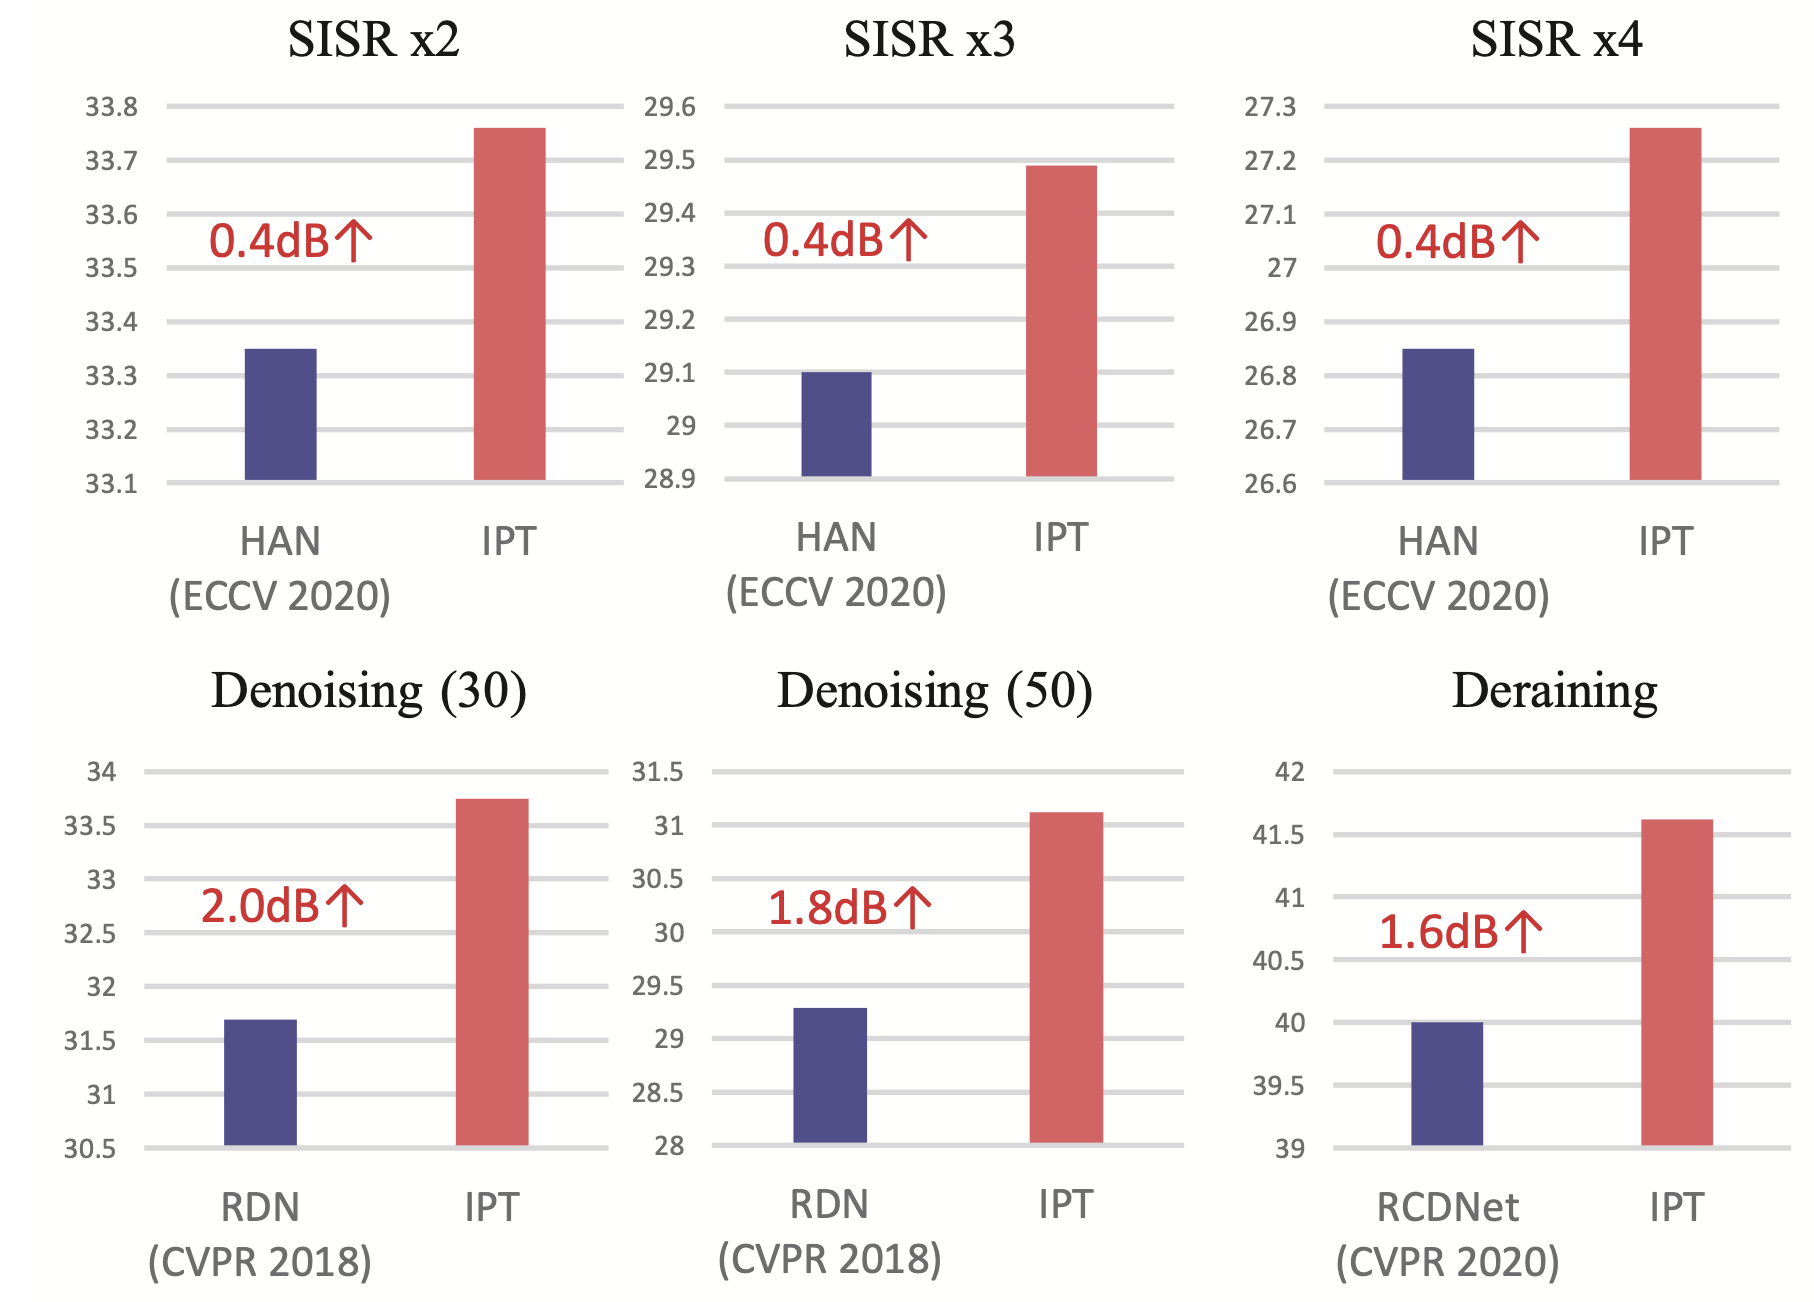
\includegraphics[width=\linewidth]{assets/comparison.png}
    \caption{\label{fig:comparison}Comparison on the performance of IPT and state-of-the-art image processing models on different tasks.}
\end{figure}

\begin{figure}[t]
    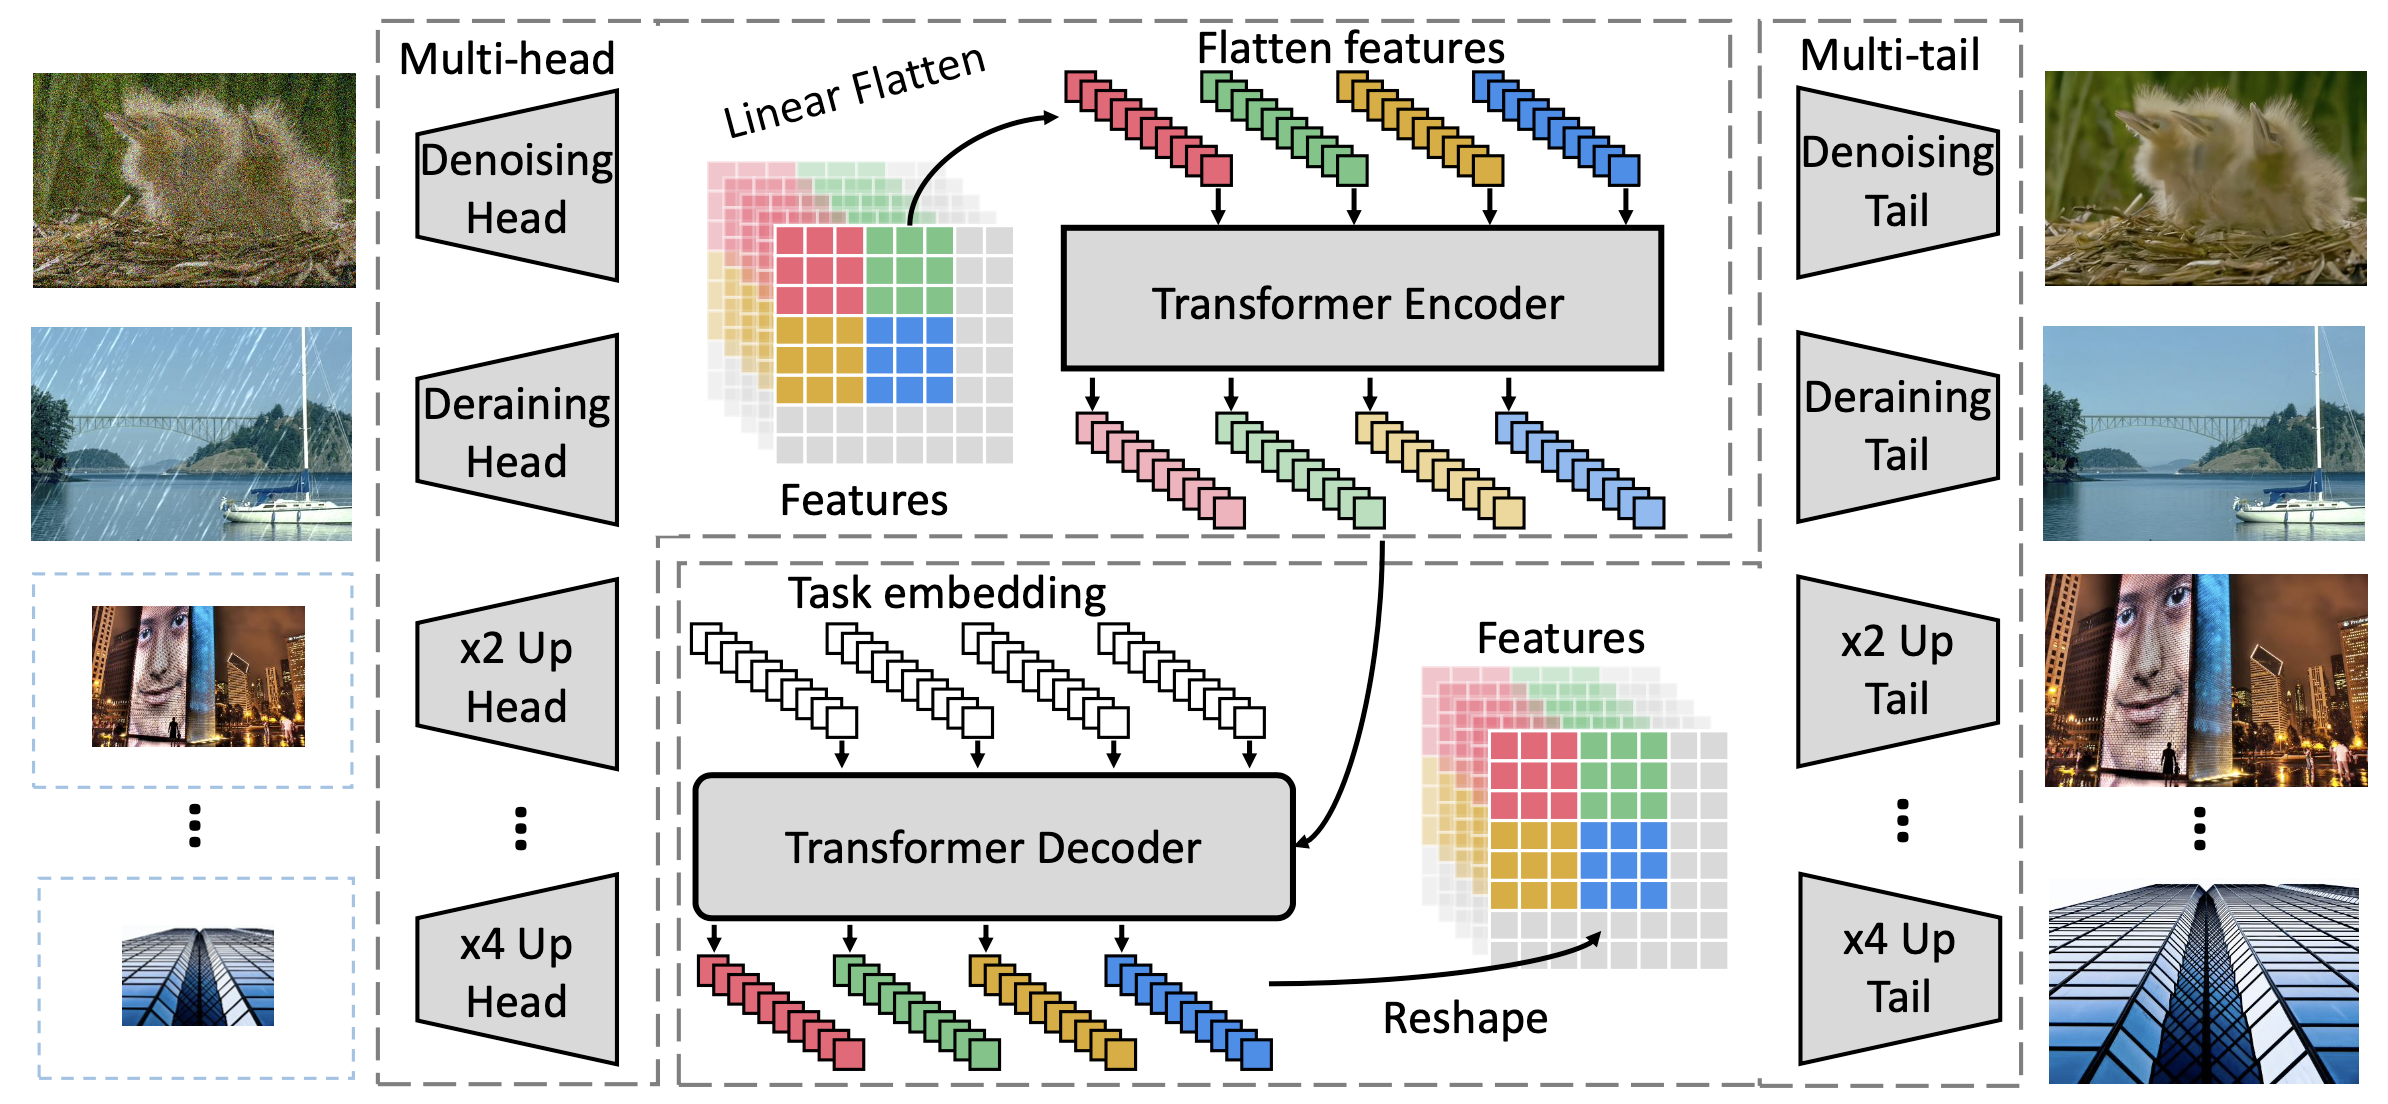
\includegraphics[width=\linewidth]{assets/ipt.png}
    \caption{\label{fig:overview}The overall pipeline of IPT. IPT consists of multi-head and multi-tail for different tasks and a shared Transformer body including encoder and decoder.}
\end{figure}




{\small
\bibliographystyle{ieee}
\bibliography{egbib}
}

\end{document}
